\section{ALGORITHM DESIGN}

\subsection{Problem $\rightarrow$ Algorithm Mapping}

\subsubsection{Bài toán 1 — Đo lường năng lực từng từ vựng của người chơi}
\begin{tabularx}{\textwidth}{@{}l X@{}}
\toprule
\textbf{Mục} & \textbf{Nội dung} \\
\midrule
\textbf{Problem} & Hệ thống cần biết người chơi đang thành thạo từ nào và yếu từ nào, để ưu tiên ôn tập từ chưa vững. \\
\textbf{Input} & \texttt{encounter\_count} (số lần gặp từ), \texttt{correct\_count} (số lần trả lời đúng), lưu trong bảng \texttt{Player\_Vocab\_Mastery} \\
\textbf{Output} & $\text{mastery\_score} \in [0.0, 1.0]$ — điểm thành thạo của từng từ \\
\textbf{Constraints} & Từ chưa gặp lần nào không được gây lỗi chia-cho-0; điểm phải phản ánh tỉ lệ đúng thực tế, không bị overfit khi gặp ít lần \\
\textbf{Algorithm type} & Scoring / Statistical Tracking \\
\textbf{Thuật toán chọn} & Knowledge Tracing — Mastery Score \\
\textbf{Công thức} & $\text{mastery\_score} = \frac{\text{correct\_count}}{\text{encounter\_count} + 1}$ \\
\textbf{Lý do chọn} & Đơn giản, $O(1)$, phù hợp với hệ thống realtime game. Mẫu số $+1$ giải quyết cả edge case từ chưa gặp lẫn giảm nhẹ điểm để tránh overconfidence. \\
\textbf{Module} & \texttt{DatabaseManager.update\_after\_combat()} $\rightarrow$ \texttt{Player\_Vocab\_Mastery} \\
\bottomrule
\end{tabularx}

\vspace{0.5cm}

\subsubsection{Bài toán 2 — Chọn từ vựng và điều chỉnh độ khó phù hợp với từng người chơi}
\begin{tabularx}{\textwidth}{@{}l X@{}}
\toprule
\textbf{Mục} & \textbf{Nội dung} \\
\midrule
\textbf{Problem} & Mỗi lần vào trận, hệ thống phải chọn từ nào để hỏi và đặt câu hỏi ở mức khó nào để vừa thử thách, vừa không làm người chơi nản. \\
\textbf{Input} & \texttt{tier\_id} (tier quái hiện tại), \texttt{mastery\_score} từng từ trong tier, \texttt{avg\_mastery} toàn tier \\
\textbf{Output} & Một từ mục tiêu (\texttt{word}, \texttt{meaning}, \texttt{word\_id}) + chuỗi \texttt{difficulty\_instruction} gửi vào prompt AI \\
\textbf{Constraints} & Phải ưu tiên từ yếu; không được kẹt mãi một nhóm từ khi tất cả mastery bằng nhau; không tăng độ khó khi người chơi chưa sẵn sàng \\
\textbf{Algorithm type} & Priority Sampling + Rule-based Heuristic \\
\textbf{Thuật toán chọn} & DDA — Dynamic Difficulty Adjustment (2 bước) \\
\textbf{Lý do chọn} & \texttt{ORDER BY RANDOM()} thuần không đảm bảo chọn từ yếu; pool-sampling 2 bước kết hợp được cả ưu tiên (top-15 yếu nhất) lẫn ngẫu nhiên (tránh kẹt). Rule-based heuristic trên mastery đủ nhẹ cho local game, không cần ML. \\
\textbf{Module} & \texttt{DatabaseManager.get\_weakest\_vocab()} + \path{AIManager.\_resolve\_difficulty\_instruction()} \\
\bottomrule
\end{tabularx}

\paragraph{Hai tầng của DDA:}
\begin{itemize}
    \item \textbf{Tầng 1 — Chọn từ (Pool Sampling):} SQL lấy 15 từ có \texttt{mastery\_score} thấp nhất trong tier (\texttt{ORDER BY mastery\_score ASC, RANDOM() LIMIT 15}), GDScript chọn ngẫu nhiên 1 trong pool đó.
    \item \textbf{Tầng 2 — Chỉnh độ khó (Adaptive Prompt):} Đọc \texttt{mastery\_score} của từ được chọn và \texttt{avg\_mastery} toàn tier, ánh xạ sang chỉ thị ngôn ngữ nhét vào prompt Ollama.
\end{itemize}

\begin{table}[h!]
\centering
\small
\begin{tabularx}{\textwidth}{@{}l X@{}}
\toprule
\textbf{Điều kiện} & \textbf{Chỉ thị gửi cho AI} \\
\midrule
$\text{encounter\_count} = 0$ & Câu hỏi nhận diện nghĩa trực tiếp, đáp án sai rõ ràng \\
$\text{mastery} < 0.3$ & Củng cố nghĩa cơ bản, không tăng độ khó \\
$0.3 \le \text{mastery} < 0.6$ & Câu trung bình, đồng/trái nghĩa \\
$0.3 \le \text{mastery} < 0.6 \text{ + tier\_is\_advanced}$ & Điền vào chỗ trống, ngữ cảnh phong phú \\
$\text{mastery} \ge 0.6$ & Sắc thái nghĩa (nuance), đáp án sai tinh tế \\
\bottomrule
\end{tabularx}
\end{table}

\newpage

\subsubsection{Bài toán 3 — Sinh câu hỏi không gây trễ (latency = 0) khi vào trận}
\begin{tabularx}{\textwidth}{@{}l X@{}}
\toprule
\textbf{Mục} & \textbf{Nội dung} \\
\midrule
\textbf{Problem} & Ollama chạy local tốn 3–10 giây mỗi request. Nếu sinh câu hỏi theo yêu cầu, người chơi phải chờ trước mỗi trận — UX tệ. \\
\textbf{Input} & \texttt{current\_tier\_id}, \texttt{is\_generating} flag, \texttt{question\_queues[tier\_id]}, $\text{MAX\_QUEUE\_SIZE} = 5$ \\
\textbf{Output} & Câu hỏi MCQ JSON lấy tức thì từ RAM (\texttt{question\_queues[tier\_id].pop\_front()}) \\
\textbf{Constraints} & Ollama chỉ xử lý 1 request tại 1 thời điểm; cần đảm bảo queue không rỗng khi vào trận; phải có fallback khi AI lỗi \\
\textbf{Algorithm type} & Producer-Consumer Queue + Priority Scheduling \\
\textbf{Thuật toán chọn} & \textbf{Asynchronous Pre-generation Engine với Multi-tier Queue} \\
\textbf{Lý do chọn} & Queue riêng theo tier thay vì queue chung giải quyết được vấn đề latency khi chuyển tier; priority scheduling (ưu tiên nạp tier hiện tại) đảm bảo không bao giờ trống khi cần. \\
\textbf{Module} & \texttt{AIManager.check\_and\_fill\_all\_queues()}, \texttt{AIManager.get\_question()} \\
\bottomrule
\end{tabularx}

\paragraph{Chiến lược ưu tiên nạp queue:}
\begin{itemize}
    \item \textbf{Ưu tiên 1} — Nạp tier hiện tại người chơi đang dùng (đảm bảo không trống khi vào trận).
    \item \textbf{Ưu tiên 2} — Nạp ngầm các tier còn thiếu theo thứ tự trong \texttt{MANAGED\_TIERS}.
    \item \textbf{Fallback} — Nếu queue rỗng: trả câu hardcode với $\text{word\_id} = -1$; \texttt{DatabaseManager} nhận diện để bỏ qua ghi mastery, tránh dữ liệu rác.
    \item \textbf{Auto-retry} — Khi AI lỗi ($\text{response\_code} \neq 200$ hoặc JSON hỏng): chờ 2 giây rồi tự gọi lại, không cần can thiệp thủ công.
\end{itemize}

\vspace{0.5cm}

\subsubsection{Bài toán 4 — Ràng buộc mô hình ngôn ngữ sinh output đúng format JSON}
\begin{tabularx}{\textwidth}{@{}l X@{}}
\toprule
\textbf{Mục} & \textbf{Nội dung} \\
\midrule
\textbf{Problem} & Qwen2.5-3B chạy local có độ tin cậy thấp hơn cloud model — dễ sinh text tự do thay vì JSON chuẩn, gây crash khi parse. \\
\textbf{Input} & \texttt{word}, \texttt{meaning}, \texttt{difficulty\_instruction}, JSON schema mong muốn \\
\textbf{Output} & Object JSON hợp lệ: \texttt{\{ question, A, B, C, D, correct\_answer, explanation \}} \\
\textbf{Constraints} & Model có thể thêm text ngoài JSON; có thể bọc trong markdown fence; response là 2 lớp JSON lồng nhau (Ollama wrapper + nội dung AI) \\
\textbf{Algorithm type} & Structured Output Engineering + Defensive Parsing \\
\textbf{Thuật toán chọn} & \textbf{4-part Structured Prompt + Double-parse + Validation} \\
\textbf{Lý do chọn} & Kết hợp ràng buộc tại cấp model (format: json của Ollama) và cấp prompt (khai báo schema tường minh, cấm text ngoài JSON) tạo 2 lớp bảo vệ. Double-parse và validation trước khi append vào queue đảm bảo không crash game dù AI có trả output hỏng. \\
\textbf{Module} & \texttt{AIManager.\_build\_prompt()}, \texttt{AIManager.\_on\_request\_completed()} \\
\bottomrule
\end{tabularx}

\paragraph{Cấu trúc prompt 4 phần:}
\begin{enumerate}
    \item \textbf{Role} — Neo AI vào bối cảnh: "Bạn là Elaria, hệ thống tạo thử thách tiếng Anh cho game RPG."
    \item \textbf{Target word} — Từ bắt buộc phải xuất hiện trong câu hỏi: \texttt{word} + \texttt{meaning}.
    \item \textbf{Difficulty instruction} — Output của \texttt{\_resolve\_difficulty\_instruction()} từ DDA.
    \item \textbf{Output rules} — Khai báo JSON schema, cấm thêm bất kỳ text nào ngoài JSON.
\end{enumerate}

\paragraph{Double-parse pipeline:}
\noindent Ollama response \\
\hspace*{1.5em}\ding{227} Parse lớp ngoài $\rightarrow$ \{ message: \{ content: '...' \} \} \\
\hspace*{3.0em}\ding{227} Parse lớp trong $\rightarrow$ \{ question, A, B, C, D, correct\_answer, explanation \} \\
\hspace*{4.5em}\ding{227} Validate: has('question') AND has('correct\_answer') AND word\_id $\neq$ -1 \\
\hspace*{6.0em}\ding{227} Append vào question\_queues[tier\_id] \hspace{0.5em} \textcolor{green}{\ding{51}} \\
\hspace*{6.0em}\ding{227} Discard nếu validate fail \hspace{5.5em} \textcolor{red}{\ding{55}} (không crash)

\newpage

\subsection{Input – Output Specification (tổng hợp)}

\begin{table}[h!]
\centering
\small
\begin{tabularx}{\textwidth}{@{}c l X X@{}}
\toprule
\textbf{\#} & \textbf{Bài toán} & \textbf{Input} & \textbf{Output} \\
\midrule
1 & Knowledge Tracing & \texttt{encounter\_count, correct\_count} & $\text{mastery\_score} \in [0.0, 1.0]$ \\
2 & DDA — Chọn từ & \texttt{tier\_id}, bảng \texttt{Player\_Vocab\_Mastery} & \texttt{word\_id, word, meaning} \\
2 & DDA — Chỉnh độ khó & \texttt{mastery\_score, avg\_mastery, encounter\_count} & \texttt{difficulty\_instruction} (string) \\
3 & Async Pre-gen & \texttt{tier\_id}, Ollama endpoint & MCQ JSON trong RAM queue \\
4 & Prompt Engineering & \texttt{word, meaning, difficulty\_instruction} & \texttt{{question, A, B, C, D, correct\_answer, explanation }} \\
\bottomrule
\end{tabularx}
\end{table}

\subsection{Core Algorithms}

\subsubsection{Algorithm 1 — Knowledge Tracing (Mastery Score)}
\textbf{Ý tưởng:} Mỗi từ vựng cần được gắn một điểm số phản ánh mức độ thành thạo thực sự của người chơi. Thay vì chỉ lưu tỉ lệ đúng đơn thuần (\texttt{correct}/\texttt{encounter}), mẫu số được cộng thêm 1 để xử lý đồng thời hai edge case: từ chưa gặp lần nào (tránh chia cho 0) và từ mới gặp ít lần nhưng luôn đúng (giảm nhẹ điểm để không overfit). Mỗi lượt chiến đấu đều cập nhật tức thì vào SQLite qua UPSERT, đảm bảo DDA luôn đọc được trạng thái mới nhất.

\paragraph{Pseudocode:}
\begin{lstlisting}
FUNCTION update_after_combat(save_id, word_id, is_correct):
    IF word_id == -1:
        RETURN  -- bo qua cau fallback, khong ghi du lieu rac

    record = DB.query(
        "SELECT encounter_count, correct_count
         FROM Player_Vocab_Mastery
         WHERE save_id = ? AND word_id = ?"
    )

    IF record EXISTS:
        new_encounter = record.encounter_count + 1
        new_correct   = record.correct_count + (1 IF is_correct ELSE 0)
        DB.execute(
            "UPDATE Player_Vocab_Mastery
             SET encounter_count = ?, correct_count = ?
             WHERE save_id = ? AND word_id = ?"
        )
    ELSE:
        DB.execute(
            "INSERT INTO Player_Vocab_Mastery
             (save_id, word_id, encounter_count, correct_count)
             VALUES (?, ?, 1, ?)"
        )

    mastery_score = new_correct / (new_encounter + 1)
    RETURN mastery_score


FUNCTION get_mastery(save_id, word_id):
    record = DB.query(...)
    IF NOT record EXISTS:
        RETURN 0.0  -- tu chua gap -> mastery mac dinh = 0
    RETURN record.correct_count / (record.encounter_count + 1)
\end{lstlisting}

\textbf{Complexity:}

\begin{table}[H]
\centering
\small
\begin{tabularx}{\textwidth}{@{}l c c X@{}}
\toprule
\textbf{Thao tác} & \textbf{Time} & \textbf{Space} & \textbf{Ghi chú} \\
\midrule
\texttt{update\_after\_combat()} & $O(1)$ & $O(1)$ & UPSERT trên PK kép (\texttt{save\_id, word\_id}) \\
\texttt{get\_mastery()} & $O(1)$ & $O(1)$ & Point lookup trên indexed PK \\
Tính \texttt{mastery\_score} & $O(1)$ & $O(1)$ & Phép chia đơn giản \\
\bottomrule
\end{tabularx}
\end{table}

\textbf{Activity Diagram} - \texttt{update\_after\_combat()}:
\begin{figure}[H]
	\centering
    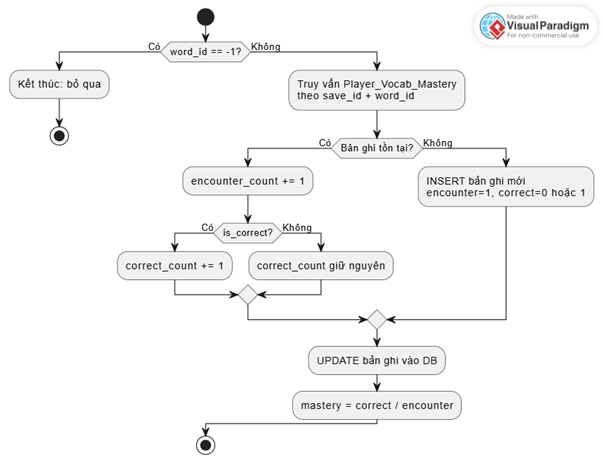
\includegraphics[scale=1]{Figure/algorithm1.png}
    \label{fig:al1}
\end{figure}

\subsubsection{Algorithm 2 — DDA Pool Sampling (chọn từ yếu nhất)}
\textbf{Ý tưởng:} Bài toán chọn từ để hỏi cần cân bằng hai mục tiêu xung đột: luôn ưu tiên từ yếu nhất (để học hiệu quả) nhưng không bị kẹt lặp lại mãi một từ (UX tệ). Giải pháp 2 bước: SQL lọc ra pool 15 từ yếu nhất trong tier (đảm bảo $100\%$ chọn từ nhóm yếu), sau đó GDScript chọn ngẫu nhiên 1 trong pool đó (đảm bảo không bị kẹt). \texttt{RANDOM()} làm tiebreaker trong SQL xử lý trường hợp tất cả mastery bằng 0 khi người chơi mới bắt đầu.

\paragraph{Pseudocode:}
\begin{lstlisting}
FUNCTION get_weakest_vocab(save_id, tier_id):
    POOL_SIZE = 15

    -- Buoc 1 (SQL): lay pool tu yeu nhat trong tier
    pool = DB.query("""
        SELECT v.word_id, v.word, v.meaning,
               COALESCE(m.correct_count * 1.0 / (m.encounter_count + 1), 0.0)
               AS mastery_score
        FROM   Vocabulary_Bank v
        LEFT JOIN Player_Vocab_Mastery m
               ON v.word_id = m.word_id AND m.save_id = ?
        WHERE  v.tier_id = ?
        ORDER BY mastery_score ASC, RANDOM()
        LIMIT ?
    """, [save_id, tier_id, POOL_SIZE])

    IF pool IS EMPTY:
        RETURN null

    -- Buoc 2 (GDScript): chon ngau nhien trong pool
    chosen = pool[ RANDOM_INT(0, pool.size() - 1) ]
    RETURN chosen  -- { word_id, word, meaning, mastery_score }
\end{lstlisting}

\textbf{Complexity}
\begin{table}[H]
\centering
\small
\begin{tabularx}{\textwidth}{@{}l c c X@{}}
\toprule
\textbf{Thao tác} & \textbf{Time} & \textbf{Space} & \textbf{Ghi chú} \\
\midrule
SQL query + LEFT JOIN & $O(n \log n)$ & $O(n)$ & $n =$ số từ trong tier; SQLite sort trên indexed \texttt{tier\_id} + \texttt{mastery\_score} \\
LIMIT 15 cắt kết quả & $O(1)$ & $O(1)$ & Pool cố định 15 phần tử \\
Random pick trong pool & $O(1)$ & $O(1)$ & Index ngẫu nhiên vào array 15 phần tử \\
\textbf{Tổng thực tế} & $\mathbf{O(n \log n)}$ & $\mathbf{O(15) \approx O(1)}$ & $n \le \sim50$ từ/tier $\rightarrow$ negligible \\
\bottomrule
\end{tabularx}
\end{table}

\textbf{Activity Diagram} - \texttt{get\_weakest\_vocab()}:
\begin{figure}[H]
	\centering
	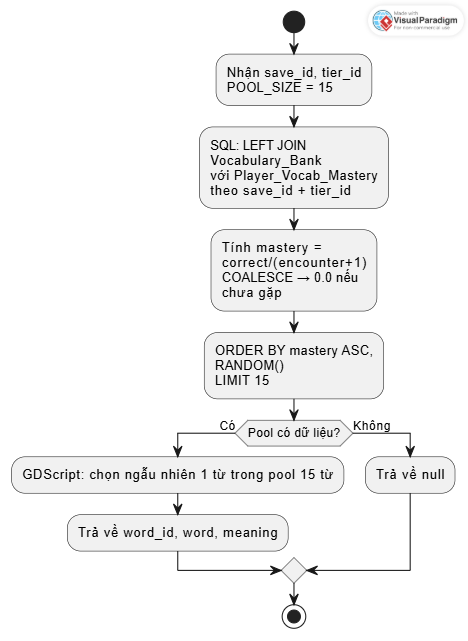
\includegraphics[scale=1]{Figure/algorithm2.png}
	\label{fig:al2}
\end{figure}

\subsubsection{Algorithm 3 — DDA Adaptive Prompt (điều chỉnh độ khó)}
\textbf{Ý tưởng:} Sau khi chọn được từ mục tiêu, hệ thống cần quyết định đặt câu hỏi ở mức khó nào phù hợp với trạng thái học hiện tại. Rule-based heuristic trên \texttt{mastery\_score} và \texttt{avg\_mastery} toàn tier đủ nhẹ cho local game và cho kết quả tức thì — không cần ML model. \texttt{tier\_is\_advanced} là biến ngưỡng giúp toàn bộ tier nâng bậc khi người chơi đã quen đủ từ vựng chung.

\paragraph{Pseudocode:}
\begin{lstlisting}
FUNCTION resolve_difficulty_instruction(word_id, save_id, tier_id):
    record      = get_vocab_record(save_id, word_id)
    encounter   = record.encounter_count  IF record EXISTS  ELSE 0
    mastery     = record.mastery_score    IF record EXISTS  ELSE 0.0
    avg_mastery = get_tier_avg_mastery(save_id, tier_id)

    THRESHOLD_HARD = 0.4
    tier_is_advanced = (avg_mastery >= THRESHOLD_HARD)

    IF encounter == 0:
        RETURN "Lan dau gap: cau hoi nhan dien nghia truc tiep, dap an sai ro rang"

    IF mastery < 0.3:
        RETURN "Hay sai: cung co nghia co ban, khong tang do kho"

    IF mastery < 0.6 AND tier_is_advanced:
        RETURN "Dang tien bo, tier kha: dong/trai nghia, dien vao cho trong nguoc canh phong phu"

    IF mastery < 0.6:
        RETURN "Dang tien bo: cau hoi muc trung binh, dong/trai nghia"

    RETURN "Thanh thao: sac thai nghia (nuance), dap an sai tinh te kho loai tru"


FUNCTION get_tier_avg_mastery(save_id, tier_id):
    result = DB.query("""
        SELECT AVG(COALESCE(m.correct_count * 1.0 / (m.encounter_count + 1), 0.0))
        FROM   Vocabulary_Bank v
        LEFT JOIN Player_Vocab_Mastery m
               ON v.word_id = m.word_id AND m.save_id = ?
        WHERE  v.tier_id = ?
    """)
    RETURN result  -- float
\end{lstlisting}

\newpage

\textbf{Complexity:}
\begin{table}[H]
\centering
\small
\begin{tabularx}{\textwidth}{@{}l c c X@{}}
\toprule
\textbf{Thao tác} & \textbf{Time} & \textbf{Space} & \textbf{Ghi chú} \\
\midrule
\texttt{get\_tier\_avg\_mastery()} & $O(n)$ & $O(1)$ & Quét toàn bộ $n$ từ trong tier để tính AVG \\
Rule matching & $O(1)$ & $O(1)$ & Chuỗi if-else cố định, không phụ thuộc $n$ \\
\textbf{Tổng} & $\mathbf{O(n)}$ & $\mathbf{O(1)}$ & $n \le \sim50$ từ/tier \\
\bottomrule
\end{tabularx}
\end{table}

\textbf{Activity Diagram} - \texttt{resolve\_difficulty\_instruction()}:
\begin{figure}[H]
	\centering
	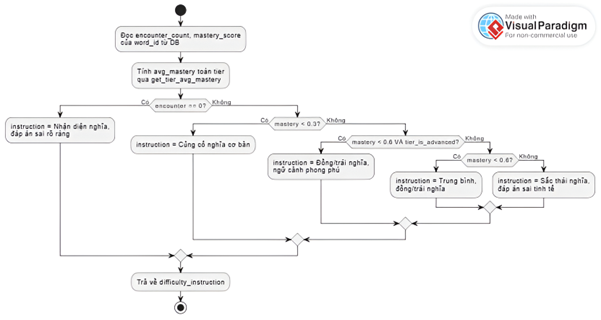
\includegraphics[scale=1]{Figure/algorithm3.png}
	\label{fig:al3}
\end{figure}

\subsubsection{Algorithm 4 — Asynchronous Pre-generation Engine}
\textbf{Ý tưởng:} Producer-Consumer pattern với multi-tier queue. \texttt{AIManager} đóng vai producer chạy ngầm, liên tục nạp câu hỏi vào \texttt{question\_queues[tier\_id]} trước khi người chơi cần. \texttt{BattleScene} đóng vai consumer, lấy tức thì từ RAM — không cần chờ AI. Flag \texttt{is\_generating} đảm bảo Ollama không nhận quá 1 request song song. Priority scheduling ưu tiên tier hiện tại. Fallback $\text{word\_id} = -1$ và auto-retry 2 giây xử lý mọi lỗi runtime mà không crash game.

\paragraph{Pseudocode:}
\begin{lstlisting}
-- Cau truc du lieu
question_queues = { 1: [], 2: [] }   -- Dictionary of Arrays
MANAGED_TIERS   = [1, 2]
MAX_QUEUE_SIZE  = 5
is_generating   = false
current_tier_id = 1


FUNCTION get_question():
    queue = question_queues[current_tier_id]
    IF queue IS EMPTY:
        check_and_fill_all_queues()   -- kich hoat nap khan cap
        RETURN build_fallback_question()  -- word_id = -1, tra ngay

    question = queue.pop_front()
    check_and_fill_all_queues()  -- nap lai ngam sau khi rut
    RETURN question


FUNCTION check_and_fill_all_queues():
    IF is_generating:
        RETURN  -- Ollama dang ban, khong gui them

    -- Uu tien 1: nap tier hien tai nguoi choi dang dung
    IF question_queues[current_tier_id].size() < MAX_QUEUE_SIZE:
        generate_question_for_tier(current_tier_id)
        RETURN

    -- Uu tien 2: nap ngam cac tier con thieu
    FOR tier IN MANAGED_TIERS:
        IF question_queues[tier].size() < MAX_QUEUE_SIZE:
            generate_question_for_tier(tier)
            RETURN


FUNCTION generate_question_for_tier(tier_id):
    is_generating = true
    vocab  = DatabaseManager.get_weakest_vocab(save_id, tier_id)
    prompt = build_prompt(vocab, resolve_difficulty_instruction(...))

    response = await Ollama.request(prompt)  -- async HTTP

    IF response.code != 200 OR JSON invalid:
        is_generating = false
        wait(2 seconds)
        check_and_fill_all_queues()  -- auto-retry
        RETURN

    question = parse_response(response)  -- double-parse
    IF question IS VALID:
        question_queues[tier_id].append(question)

    is_generating = false
    check_and_fill_all_queues()  -- nap tiep nhe neu con thieu


FUNCTION build_fallback_question():
    RETURN {
        word_id: -1,
        question: "What does 'Forest' mean?",
        A: "Rung", B: "Bien", C: "Nui", D: "Dong",
        correct_answer: "A",
        explanation: "Forest = Rung (cau du phong)"
    }
\end{lstlisting}

\newpage

\textbf{Complexity:}
\begin{table}[H]
\centering
\small
\begin{tabularx}{\textwidth}{@{}l c c X@{}}
\toprule
\textbf{Thao tác} & \textbf{Time} & \textbf{Space} & \textbf{Ghi chú} \\
\midrule
\texttt{get\_question()} từ RAM & $O(1)$ & $O(1)$ & Pop từ đầu array \\
\texttt{check\_and\_fill\_all\_queues()} & $O(T)$ & $O(1)$ & $T = $ số tier ($T=2$, hằng số) \\
Queue RAM tổng & — & $O(T \times K)$ & $2 \text{ tier} \times 5 \text{ câu} = 10 \text{ objects} \rightarrow O(1)$ \\
Latency khi tier switch & $O(1)$ & $O(1)$ & Chỉ cập nhật \texttt{current\_tier\_id} \\
AI generation (Ollama) & $O(1)^*$ & $O(1)$ & $^*3\text{--}10$ giây wall-clock chạy bất đồng bộ \\
\bottomrule
\end{tabularx}
\end{table}

\textbf{Activity Diagram} - \texttt{get\_question()} + \texttt{check\_and\_fill\_all\_queues()}:
\begin{figure}[H]
	\centering
	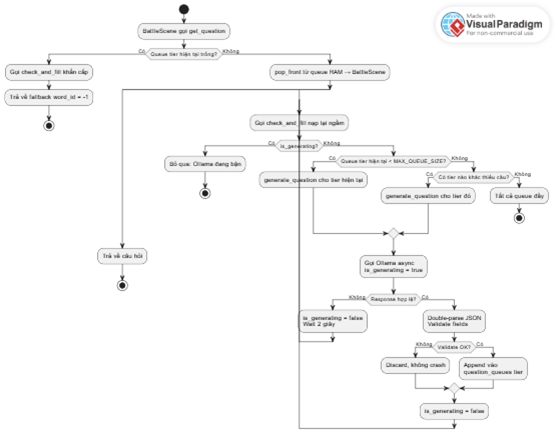
\includegraphics[scale=1]{Figure/algorithm4.png}
	\label{fig:al4}
\end{figure}

\paragraph{PlantUML Activity Diagram — get\_question() + check\_and\_fill\_all\_queues():}
\begin{lstlisting}
@startuml
start
:BattleScene goi get_question;
if (Queue tier hien tai trong?) then (Co)
    :Goi check_and_fill khan cap;
    :Tra ve fallback word_id = -1;
    stop
else (Khong)
    :pop_front tu queue RAM -> BattleScene;
    split
        :Tra ve cau hoi;
        stop
    split again
        label quay_lai_nap_ngam
        :Goi check_and_fill nap lai ngam;
        if (is_generating?) then (Co)
            :Bo qua: Ollama dang ban;
            stop
        else (Khong)
            if (Queue tier hien tai < MAX_QUEUE_SIZE?) then (Co)
                :generate_question cho tier hien tai;
            else (Khong)
                if (Co tier nao khac thieu cau?) then (Co)
                    :generate_question cho tier do;
                else (Khong)
                    :Tat ca queue day;
                    stop
                endif
            endif
            :Goi Ollama async\nis_generating = true;
            if (Response hop le?) then (Khong)
                :is_generating = false\nWait 2 giay;
                goto quay_lai_nap_ngam
            else (Co)
                :Double-parse JSON\nValidate fields;
                if (Validate OK?) then (Khong)
                    :Discard, khong crash;
                else (Co)
                    :Append vao\nquestion_queues tier;
                endif
                :is_generating = false;
                goto quay_lai_nap_ngam
            endif
        endif
    end split
endif
@enduml
\end{lstlisting}

\subsubsection{Algorithm 5 — Structured Prompt Engineering \& Double-parse}
\textbf{Ý tưởng:} Qwen2.5-3B chạy local không ổn định bằng cloud model. Chiến lược phòng thủ 2 lớp: lớp 1 ràng buộc output tại cấp model (tham số \texttt{format: json} của Ollama API) và cấp prompt (khai báo schema tường minh, cấm text ngoài JSON); lớp 2 là pipeline parse-validate-discard trong code để không bao giờ crash dù AI trả output hỏng. $\text{word\_id} = -1$ là sentinel value cho phép toàn bộ pipeline nhận biết câu fallback mà không cần điều kiện đặc biệt ở mỗi bước.

\paragraph{Pseudocode:}
\begin{lstlisting}
FUNCTION build_prompt(vocab, difficulty_instruction):
    RETURN """
    [ROLE]
    Ban la Elaria, he thong tao thu thach tieng Anh cho game RPG rung.

    [TARGET WORD]
    Tu: {vocab.word}
    Nghia: {vocab.meaning}

    [DIFFICULTY INSTRUCTION]
    {difficulty_instruction}

    [OUTPUT RULES]
    Tra ve JSON hop le voi dung cac truong sau, khong them text nao khac:
    {
        "question":       "<cau hoi trac nghiem>",
        "A":              "<dap an A>",
        "B":              "<dap an B>",
        "C":              "<dap an C>",
        "D":              "<dap an D>",
        "correct_answer": "<A hoac B hoac C hoac D>",
        "explanation":    "<giai thich ngan tai sao dap an dung>"
    }
    """


FUNCTION parse_and_validate(raw_response, word_id):
    TRY:
        -- Lop 1: parse Ollama wrapper
        outer = JSON.parse(raw_response)
        content_str = outer["message"]["content"]

        -- Lop 2: parse JSON cau hoi do AI sinh
        q_data = JSON.parse(content_str)

        -- Validate bat buoc
        IF NOT q_data.has("question"):       RETURN null
        IF NOT q_data.has("correct_answer"): RETURN null
        IF word_id == -1:                RETURN null

        q_data["word_id"] = word_id
        RETURN q_data

    CATCH any error:
        RETURN null  -- discard silently, khong crash


FUNCTION _on_ollama_response(response):
    IF response.code != 200:
        handle_error()
        RETURN

    question = parse_and_validate(response.body, current_word_id)
    IF question IS NOT null:
        question_queues[current_tier_id].append(question)
\end{lstlisting}

\textbf{Complexity:}
\begin{table}[H]
\centering
\small
\begin{tabularx}{\textwidth}{@{}l c c X@{}}
\toprule
\textbf{Thao tác} & \textbf{Time} & \textbf{Space} & \textbf{Ghi chú} \\
\midrule
\texttt{build\_prompt()} & $O(1)$ & $O(L)$ & $L =$ độ dài prompt, hằng số \\
\texttt{JSON.parse()} lần 1 & $O(R)$ & $O(R)$ & $R =$ kích thước response ($\sim500$ chars) \\
\texttt{JSON.parse()} lần 2 & $O(C)$ & $O(C)$ & $C =$ kích thước content ($\sim300$ chars) \\
Validate (\texttt{has}-check) & $O(1)$ & $O(1)$ & 2 key lookup cố định \\
\textbf{Tổng} & $\mathbf{O(R)}$ & $\mathbf{O(R)}$ & $R$ nhỏ, thực tế negligible \\
\bottomrule
\end{tabularx}
\end{table}

\textbf{Activity Diagram - build $\rightarrow$ request $\rightarrow$ double-parse $\rightarrow$ validate} 
\begin{figure}[H]
	\centering
	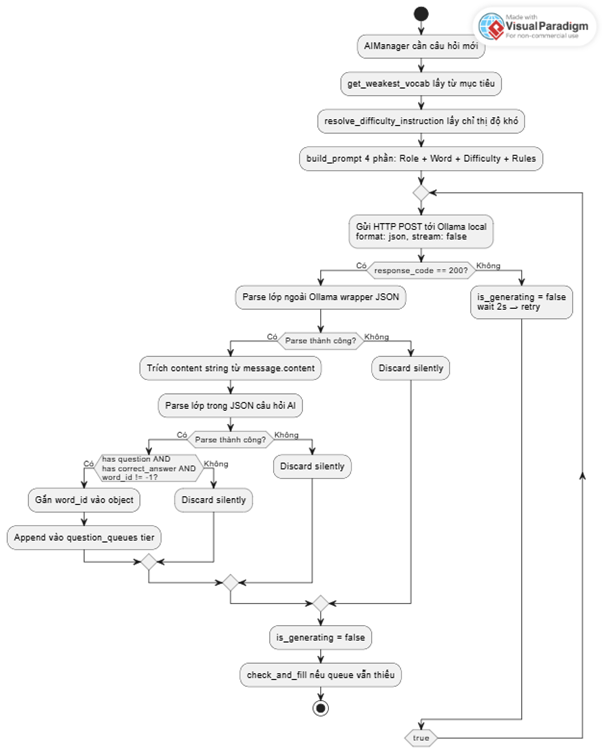
\includegraphics[scale=1]{Figure/algorithm5.png}
	\label{fig:al5}
\end{figure}


\textbf{Tóm tắt complexity của 5 thuật toán cốt lõi:}
\begin{table}[H]
\centering
\small
\begin{tabularx}{\textwidth}{@{}c l c c@{}}
\toprule
\textbf{\#} & \textbf{Thuật toán} & \textbf{Time} & \textbf{Space} \\
\midrule
1 & Knowledge Tracing (mastery score) & $O(1)$ & $O(1)$ \\
2 & DDA Pool Sampling & $O(n \log n)$ & $O(1)$ \\
3 & DDA Adaptive Prompt & $O(n)$ & $O(1)$ \\
4 & Async Pre-generation Engine & $O(1)$ runtime / $O(T \times K)$ build & $O(T \times K)$ \\
5 & Structured Prompt + Double-parse & $O(R)$ & $O(R)$ \\
\bottomrule
\end{tabularx}
\caption*{Với $n \le 50$ từ/tier, $T = 2$ tier, $K = 5$ câu/queue, $R \approx 500$ ký tự — tất cả đều negligible về mặt thực tế.}
\end{table}

\subsection{Optimization Strategy}
Phần này trình bày các chiến lược tối ưu hóa được áp dụng cho từng tầng của hệ thống, từ cơ sở dữ liệu, thuật toán lõi, đến pipeline sinh câu hỏi AI. Mỗi chiến lược đều xuất phát từ một vấn đề thực tế quan sát được trong quá trình phát triển, không phải tối ưu hóa lý thuyết thuần túy.

\subsubsection{Phần 1 — Cơ sở dữ liệu (SQLite)}
\textbf{Vấn đề:} Hàm \texttt{get\_weakest\_vocab()} được gọi trước mỗi lần sinh câu hỏi. Nếu query chạy chậm, toàn bộ pipeline AI bị trì hoãn theo.

\paragraph{Chiến lược áp dụng:}
\begin{itemize}
    \item \textbf{Composite Index trên (save\_id, tier\_id):}
    Query cốt lõi của DDA lọc đồng thời theo hai cột \texttt{save\_id} và \texttt{tier\_id}. Không có index, SQLite phải quét toàn bộ bảng \texttt{Player\_Vocab\_Mastery} mỗi lần gọi. Composite index cho phép SQLite nhảy thẳng đến đúng partition dữ liệu:
\end{itemize}
\begin{lstlisting}[language=SQL]
CREATE INDEX IF NOT EXISTS idx_mastery_save_tier
ON Player_Vocab_Mastery(save_id, tier_id);
\end{lstlisting}
Với dataset nhỏ ($\sim50$ từ/tier), lợi ích chưa rõ ràng ngay, nhưng khi mở rộng lên hàng trăm từ ở các chapter sau, index này ngăn hệ số tăng trưởng query time từ $O(n)$ về $O(\log n)$.

\begin{itemize}
    \item \textbf{\texttt{COALESCE} thay vì subquery:}
    Từ chưa gặp lần nào không có bản ghi trong \texttt{Player\_Vocab\_Mastery}. Thay vì dùng subquery kiểm tra sự tồn tại (chạy hai lần), \texttt{LEFT JOIN} kết hợp \texttt{COALESCE} xử lý trong một lần duy nhất:
\end{itemize}
\begin{lstlisting}[language=SQL]
-- Khong toi uu: 2 lan truy cap DB
IF NOT EXISTS (SELECT 1 FROM mastery WHERE word_id = ?) THEN mastery = 0.0

-- Toi uu: 1 lan, NULL -> 0.0 inline
COALESCE(m.correct_count * 1.0 / (m.encounter_count + 1), 0.0) AS mastery_score
\end{lstlisting}

\begin{itemize}
    \item \textbf{\texttt{INSERT OR IGNORE} cho vocabulary seeding:}
    Hàm \texttt{\_seed\_from\_csv()} chạy mỗi lần khởi động game. Thay vì kiểm tra trước rồi mới insert (2 lần truy cập), \texttt{INSERT OR IGNORE} kết hợp với $\text{UNIQUE}(\text{word})$ constraint xử lý idempotency trong một lệnh duy nhất — đảm bảo chạy nhiều lần không sinh dữ liệu trùng, không cần thêm logic kiểm tra.
\end{itemize}

\subsubsection{Phần 2 — Thuật toán DDA}
\textbf{Vấn đề ban đầu:} \texttt{ORDER BY RANDOM()} thuần có thể chọn từ đã thành thạo nếu may mắn. Khi tất cả từ trong tier có $\text{mastery} = 0.0$ (người chơi mới), \texttt{ORDER BY mastery ASC} không phân biệt được các từ với nhau, dẫn đến hệ thống kẹt lặp lại \texttt{word\_id} 1–5 liên tục.

\paragraph{Chiến lược áp dụng:}
\begin{itemize}
    \item \textbf{Pool Sampling 2 bước thay vì random thuần:}
\end{itemize}
\begin{table}[h!]
\centering
\small
\begin{tabularx}{\textwidth}{@{}l X@{}}
\toprule
\textbf{Cách tiếp cận} & \textbf{Vấn đề} \\
\midrule
\texttt{ORDER BY RANDOM()} & Có thể chọn từ thành thạo \\
\texttt{ORDER BY mastery ASC} (chỉ lấy 1) & Kẹt \texttt{word\_id} 1–5 khi mastery bằng nhau \\
\textbf{Pool 15 + \texttt{RANDOM()} tiebreaker} & \textbf{Đảm bảo từ yếu + không kẹt} \\
\bottomrule
\end{tabularx}
\end{table}

Giải pháp cuối kết hợp được cả hai mục tiêu mà không tăng complexity đáng kể: SQL vẫn chỉ chạy một lần, GDScript chỉ thêm một phép random trên array 15 phần tử.

\begin{itemize}
    \item \textbf{$\text{pool\_size} = 15$ thay vì 5:} Tăng từ 5 lên 15 giải quyết trường hợp tier có nhiều từ cùng mastery thấp — pool lớn hơn giúp phân phối đều hơn, người chơi không cảm thấy bị hỏi lặp đi lặp lại cùng một từ trong nhiều trận liên tiếp.
    \item \textbf{\texttt{tier\_is\_advanced} như một ngưỡng toàn cục:} Thay vì đánh giá độ khó độc lập cho từng từ, biến $\text{tier\_is\_advanced} = (\text{avg\_mastery} \ge 0.4)$ cho phép toàn bộ tier "lên hạng" khi người chơi đã quen đủ từ vựng. Điều này giúp tránh tình huống một từ lẻ bị đẩy lên độ khó cao trong khi người chơi vẫn đang vật lộn với phần lớn tier đó.
\end{itemize}


\subsubsection{Phần 3 — Async Pre-generation Engine}
\textbf{Vấn đề:} Ollama chạy local tốn 3–10 giây mỗi request. Sinh câu hỏi theo yêu cầu (on-demand) buộc người chơi chờ trước mỗi trận.

\paragraph{Chiến lược áp dụng:}
\begin{itemize}
    \item \textbf{Pre-generation — sinh câu hỏi trước khi cần:} Câu hỏi được tạo sẵn trong lúc người chơi di chuyển trên bản đồ (thời gian rảnh của hệ thống), lưu vào RAM queue. Khi vào trận, \texttt{get\_question()} chỉ cần \texttt{pop\_front()} — latency bằng 0 từ góc nhìn người chơi.
    \item \textbf{Multi-tier Queue thay vì queue chung:} Queue chung có nhược điểm cơ bản: khi người chơi đổi tier, toàn bộ queue bị xóa và phải sinh lại từ đầu, gây ra 3–10 giây chờ. Dictionary of Arrays giải quyết triệt để:
\end{itemize}
\begin{lstlisting}
var question_queues: Dictionary = { 1: [], 2: [] }
\end{lstlisting}
Mỗi tier giữ queue riêng, việc đổi tier chỉ cập nhật con trỏ \texttt{current\_tier\_id} — không đụng đến dữ liệu đã cache.

\begin{itemize}
    \item \textbf{Priority Scheduling — ưu tiên tier hiện tại:} \texttt{check\_and\_fill\_all\_queues()} không nạp tất cả tier song song (Ollama chỉ xử lý 1 request tại 1 thời điểm). Thay vào đó, hàm ưu tiên tier đang dùng trước, rồi mới nạp ngầm các tier còn lại — đảm bảo queue của tier hiện tại không bao giờ trống khi người chơi cần.
    \item \textbf{Flag \texttt{is\_generating} ngăn request song song:} Ollama single-threaded không xử lý được concurrent request. Flag boolean đơn giản đủ để serialize toàn bộ pipeline:
\end{itemize}
\begin{lstlisting}
if is_generating:
    return  -- bo qua, khong gui them request
\end{lstlisting}
Chi phí: 1 biến boolean. Lợi ích: không bao giờ gây quá tải Ollama.

\begin{itemize}
    \item \textbf{Fallback + Auto-retry không cần can thiệp thủ công:} Khi AI lỗi, hệ thống không crash mà trả về câu dự phòng ($\text{word\_id} = -1$) để game tiếp tục. Sau 2 giây, \texttt{check\_and\_fill\_all\_queues()} tự gọi lại — người chơi không nhận ra bất kỳ sự gián đoạn nào.
\end{itemize}

\subsubsection{Phần 4 — Prompt Engineering}
\textbf{Vấn đề:} Qwen2.5-3B chạy local không ổn định — dễ thêm text ngoài JSON, bọc output trong markdown fence, hoặc bỏ sót field bắt buộc.

\paragraph{Chiến lược áp dụng:}
\begin{itemize}
    \item \textbf{Ràng buộc 2 lớp:} Lớp 1 tại cấp model: tham số \texttt{format: json} của Ollama API buộc model enforce JSON ở cấp tokenizer — xác suất sinh text tự do giảm đáng kể. Lớp 2 tại cấp prompt: khai báo tường minh JSON schema và cấm thêm bất kỳ text nào khác, tạo neo ngữ nghĩa cho model.
    \item \textbf{$\text{temperature} = 0.45$ — cân bằng đa dạng và ổn định:} Giá trị này được chọn sau quá trình thử nghiệm thực tế:
\end{itemize}
\begin{table}[h!]
\centering
\small
\begin{tabularx}{\textwidth}{@{}l X@{}}
\toprule
\textbf{Temperature} & \textbf{Hệ quả} \\
\midrule
$< 0.3$ & Câu hỏi lặp lại, đáp án sai quá giống nhau \\
$\mathbf{0.45}$ & \textbf{Đủ đa dạng câu hỏi, đủ ổn định để đúng JSON} \\
$> 0.7$ & Format JSON không ổn định, field hay bị thiếu \\
\bottomrule
\end{tabularx}
\end{table}

\begin{itemize}
    \item \textbf{\texttt{stream: false} — đơn giản hóa parsing:} Nhận toàn bộ response một lần thay vì xử lý stream token-by-token. Đánh đổi: người chơi không thấy câu hỏi "hiện dần", nhưng không quan trọng vì câu hỏi được pre-generate ngầm, không hiển thị trong lúc sinh.
    \item \textbf{Double-parse + validate trước khi enqueue:} Pipeline parse-validate-discard đảm bảo chỉ câu hỏi hợp lệ mới vào queue:
    \[
    \text{Parse lớp ngoài} \rightarrow \text{Parse lớp trong} \rightarrow \text{Kiểm tra 2 field bắt buộc} \rightarrow \text{Enqueue / Discard silently}
    \]
    \textit{Discard silently} — không throw exception, không crash — giúp hệ thống tự phục hồi mà không cần logic xử lý lỗi phức tạp ở tầng trên.
\end{itemize}


\subsubsection{Tổng kết các đánh đổi (Trade-offs)}
Mỗi chiến lược tối ưu hóa đều kèm theo một đánh đổi được chấp nhận có chủ đích:

\begin{table}[H]
\centering
\small
\begin{tabularx}{\textwidth}{@{}l X X@{}}
\toprule
\textbf{Chiến lược} & \textbf{Lợi ích} & \textbf{Đánh đổi chấp nhận} \\
\midrule
Multi-tier Queue & Latency = 0 khi đổi tier & RAM tăng nhẹ ($\sim2$KB) \\
Pool size = 15 & Phân phối đều, không kẹt từ & Query trả về nhiều hơn 1 bản ghi \\
\texttt{stream: false} & Parsing đơn giản & Không có hiệu ứng "hiện dần" \\
$\text{temperature} = 0.45$ & JSON ổn định & Câu hỏi ít sáng tạo hơn mức cao \\
Discard silently & Không crash khi AI lỗi & Queue có thể thiếu 1 câu tạm thời \\
Pre-generation ngầm & Người chơi không chờ AI & Câu hỏi sinh sẵn có thể không dùng đến \\
\bottomrule
\end{tabularx}
\end{table}